% Activate the following line by filling in the right side. If for example the name of the root file is Main.tex, write
% "...root = Main.tex" if the chapter file is in the same directory, and "...root = ../Main.tex" if the chapter is in a subdirectory.
 
%!TEX root =  

\chapter{Design}
\label{design}

\minitoc

\subsection*{Purpose}
This chapter describes the design phase of the program, where the program architecture is established. Several critical decisions are made in this phase and the design and architecture decisions impacts the way the implementation phase proceeds as it defines how the final software system is decomposed into modules, and how these modules behave and interact with each other. Details regarding programming languages, algorithms, data structures, coding standards and other software engineering features must also be established prior to proceeding from this phase.

\section{Development Tools and Technologies}\label{DevTools}
This section details some of the choices that were made regarding development tools and technologies for this project.

\subsection{Documents and Source Code Repositories}
For software projects of a certain scale, version control is an important technology that allows project members to work simultaneously against the same files without causing inconsistencies. Version control systems also allow for comparison with older versions, tracking changes and restoring previous copies in the case of errors.

For source code repositories and version control, \textbf{Git} was selected. Git is a distributed, open source version control system that is available for all platforms. Git is also used for hosting the \LaTeX documents that comprise this report. For other documents such as meeting minutes, agendas, status reports, time reporting and certain planning documents, \textbf{Google Docs} is used.


\subsection{Programming Languages}
\textbf{Java} is chosen as the primary programming language for implementing the majority of the code. Java is an object oriented programming language providing a level of abstraction appropriate for the task at hand in addition to a rich set of libraries, including the SWING library for GUI programming, and several libraries for networking. It also simplifies writing a browser plugin as major browsers such as Google Chrome and Firefox employ Javascript as scripting language for plugin.
Javascript was used in small measure for the use of a CouchDB community server.

\subsection{Development Tools}
Eclipse was used for all Java development, while standard text editors were used for Javascript and manual P3P policy editing. The CouchDB server was hosted on a VMware virtual machine, and was accessible via web interface on most standard web browsers.

\subsection{Databases}
For testing purposes, it has been decided on using flat file storage of privacy policy data using Java's \texttt{Serializable} interface. However, the output functionality is to be written in a generic fashion to simplify use of database systems such as MySQL, CouchDB and so forth. 

%[Discuss community server here]
[Discuss community server here]

\subsection{Third Party Libraries}
 
For developing the CBR as well as P3P parsing components of the Privacy Advisor, a decision had to be made regarding the usage of third party libraries, either for components or for the entire CBR system. Two options were considered with respect to the CBR system. The first was to use a full third party CBR system (jColibri). The alternative was to use a third party system for the retrieval component of the CBR system (i.e. a k Nearest Neighbors (kNN) implementation).


\subsubsection{Third Party CBR System}

The customer, SINTEF ICT, suggested looking into an open source CBR library developed at the Universidad Complutense de Madrid.
 
jColibri is a CBR system that has been under development for well over 10 years and is a very comprehensive system allowing for database interfaces and several other features,  and is according to the customer, a popular choice in academia for CBR projects. It is also written in Java, which of course makes interfacing it simple from our own Java project.
 
However, its comprehensiveness also means that it takes more reading to understand and properly apply to the project at hand, and due to its size and poor documentation, jColibri was ultimately deemed unfit for the Privacy Advisor project. Due to the limited time resources available to this project, the risks associated with spending a large amount of time on a third party library that eventually would not be running was to high.
 
\subsubsection{Third Party k Nearest Neighbors Implementations}
Since kNN is a standard classification algorithm, there are several open source implementations available. Limiting the search space to Java implementations, a library called \emph{The Java Machine Learning Library} (JavaML) was the primary candidate, as it provided a clean and simple interface and allowed for extracting confidence measures.
 
The problem with this library relates to the nature of distance metrics used in classifying privacy policies which is compositional in a way that is non-trivial to handle in JavaML. Furthermore, JavaML seems to operate only on arrays of floating point numbers, which means the distance metric must be defined in two stages; first mapping from \emph{policy domain} to real numbers, then in terms of a metric on real vectors.

\subsubsection{P3P/XML Parser}
Looking for XML parsers on the Java platform, we found out that there are two different types of XML parsers we could use, the first being a DOM Parsers and the second one being a sequential access parser. The difference being that DOM parsers operate on the document as a whole, while sequential access parsers operates on each piece of the XML document sequentually.

We ended up using SAXParser, an internal sequential access parsers in Java. The task from here was to implement it, making the policy as an object with the fields of our choosing. It works by sequentially going through all elements of the XML document, and with easy string comparison, checking if the element is of the wanted ones.



\section{Standards}
To achieve clean and reusable code, the project has adopted Oracle's Coding Conventions for the Java Programming Language\footnote{http://www.oracle.com/technetwork/java/codeconvtoc-136057.html}. This is mentioned in the requirements specification due to the high likelihood of the customer having to change the source code for later adaptations.


\section{Architecture}
%http://www.cmcrossroads.com/bradapp/docs/sdd.html
In implementing Privacy Advisor, a class structure is built around the CBR agent model discussed in T{\o}ndel and Nyre. Refinements needed to be made include data structures for storing policies, databases, choosing actual algorithms, and so forth. This section describes how the design in broad terms.

\begin{figure}[htbp]
\begin{center}
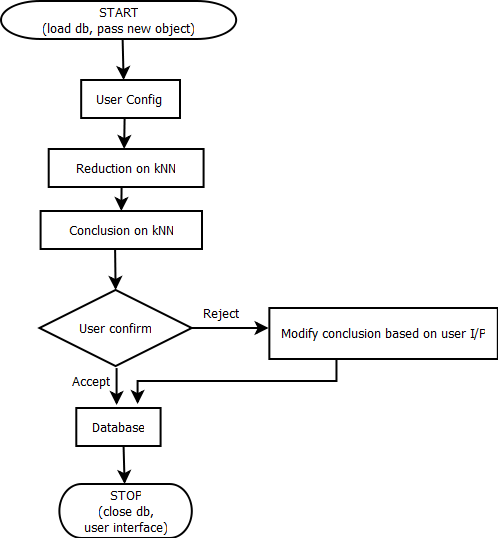
\includegraphics[width = \textwidth]{DesignReport/uml/flowchart.png}
\caption{Program Flow.}
\label{DesignFlowChrt}
\end{center}
\end{figure}

\subsection{Design Overview}
This section describes the architecture of the local CBR based system. The next section gives an overview over the design of the server component using collaborative filtering and how it interfaces with the local system.  

\begin{figure}[htbp]
\begin{center}
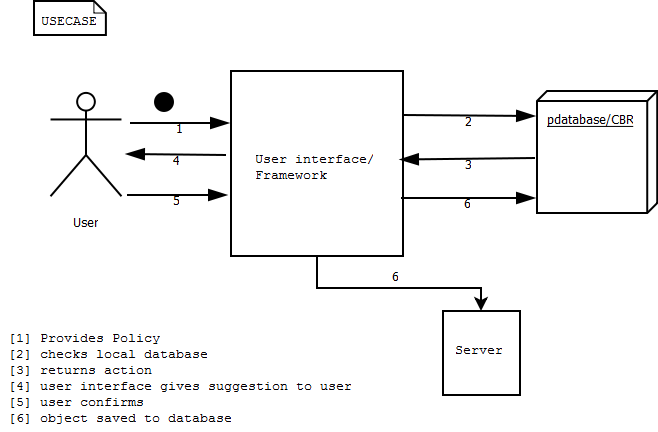
\includegraphics[width = \textwidth]{DesignReport/uml/Case.png}
\caption{System Overview.}
\label{SystemOverview}
\end{center}
\end{figure}

Figures~\ref{DesignFlowChart} and \ref{SystemOverview} illustrate the broad structure of the system; a policy object is passed to the CBR system from the user via the user interface. The CBR does a lookup on similar cases in the local database and makes a recommendation based on the similar cases and provides the user with the advice and the background for the advice through the user interface. The user can then give a feedback on the advice choosing to accept or reject it. The user feedback is then stored back to the database.

\subsubsection{CLI and I/O}
Privacy Advisor can be run using either a command line interface (CLI) or a graphical user interface (GUI). Both the CLI and the GUI are built on top of a "General Input/Output'' module, GIO. GIO creates the database objects and issues the proper commands to the CBR framework based on user input.

\begin{figure}[htbp]
\begin{center}
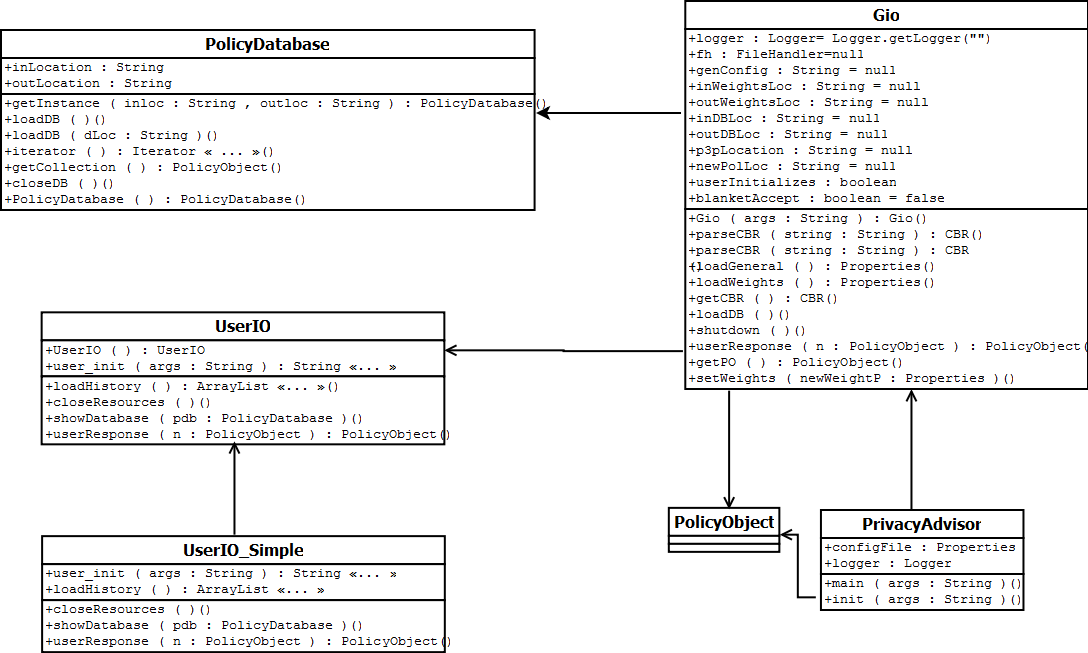
\includegraphics[width = \textwidth]{DesignReport/uml/gio.png}
\caption{working of system.}
\label{working of system}
\end{center}
\end{figure}

<<<<<<< HEAD
\subsubsection{GUI}
=======
\subsubsection{GUI} 
%TODO Einar
>>>>>>> 9390378237fe2fce259a200c1bcfc712c87aa408

\subsubsection{Weights and Configuration Files}
As an addition to passing command line arguments, GIO also reads a text based configuration file containing CBR and database settings. The configuration files are detailed in the User Documentation in table~\ref{configTable}. 

\subsubsection{CBR} % TODO Nicholas: Why PDatabase is not connected directly to CBR
Input from the UI is passed on to the CBR framework. CBR in turn references three other key modules, a \emph{reduction} algorithm, a \emph{conclusion} algorithm, and finally, a \emph{learning} algorithm.

The reduction algorithm searches the database to find the most similar cases to the new case presented. The canonical reduction algorithm is k Nearest Neighbors, discussed in section~\ref{kNN}. The conclusion algorithm looks at the set of cases returned by the reduction, and decides on the most appropriate action for the novel case. It also returns a measure of confidence in the conclusion reached.

Finally, a learning algorithm allows for automatically tuning the parameters used for distance calculations. This is discussed further in section~\ref{learnAlgos}.

An overview of the CBR system is given in Figure~\ref{cbr_fig}...
% comment reduction, learning, conclusion, KNN


\begin{figure}[htbp]
\begin{center}
\includegraphics[width = \textwidth]{DesignReport/uml/CBR.png}
\caption{CBR System.}
\label{cbr_fig}
\end{center}
\end{figure}


\subsubsection{P3P Policy Objects}
An overview of the Policy Object is given in Figure~\ref{po_fig}...
<<<<<<< HEAD
=======
%TODO Einar

>>>>>>> 9390378237fe2fce259a200c1bcfc712c87aa408

\begin{figure}[htbp]
\begin{center}
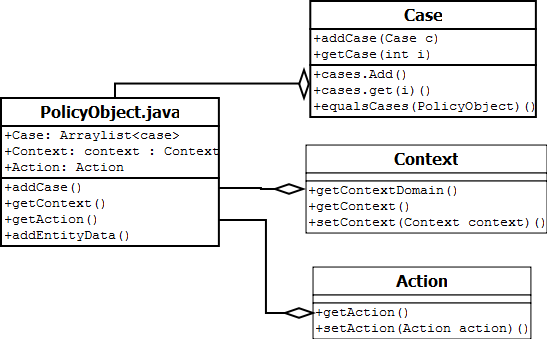
\includegraphics[width = \textwidth]{DesignReport/uml/po.png}
\caption{Policy Object.}
\label{po_fig}
\end{center}
\end{figure}

\subsubsection{P3P Policy Database}
<<<<<<< HEAD
An overview of the Policy Database is given in Figure~\ref{pd_fig}...
=======
The local case history, maintained in a local database, is stored via a concrete class implementing 'PolicyDatabase'. This abstract class details the required methods for a local policy database: a singleton constructor for the database object; a call to load the database once constructed, from disk; a method adding a single policy to the database; a method returning a Java iterator over the stored PolicyObjects, and a call to return all policies from a given domain.

In order to ensure consistency, the local policy database enforces singletonness. The database object itself is constructed without the actual history, requiring a seperate parameter-less 'loadDB' call on it to load policies from disk to the class, if necessary.

During the CBR cycle, it becomes necessary to check past cases for relevancy during the 'retrieve' phase. This is accomplished by using the standard java Iterator return by \texttt{getiterator()}.
Finally, the CBR cycle concludes by saving the new case (using 'addpolicy(newpolicy)'), and closing the database using 'closeDB()' (which is when the cases would be saved to disk).

An overview of the Policy Database is given in Figure~\ref{pd_fig}...
%TODO

>>>>>>> 9390378237fe2fce259a200c1bcfc712c87aa408

\begin{figure}[htbp]
\begin{center}
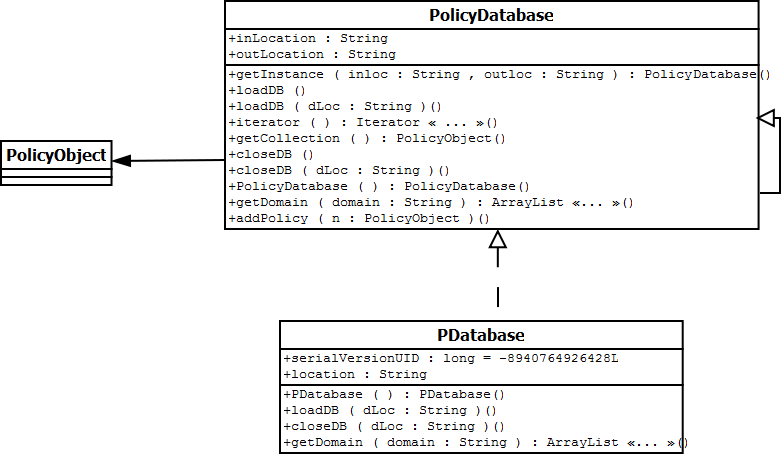
\includegraphics[width = \textwidth]{DesignReport/uml/pd.png}
\caption{Policy Database.}
\label{pd_fig}
\end{center}
\end{figure}

\subsection{Interfaces}

% \begin{center}
%   \begin{table}[htdp]
%     \begin{tabularx}{\textwidth}{ | X | |}
      
%     \end{tabularx}
%   \end{table}
% \end{center}



\begin{figure}[htbp]
\begin{center}
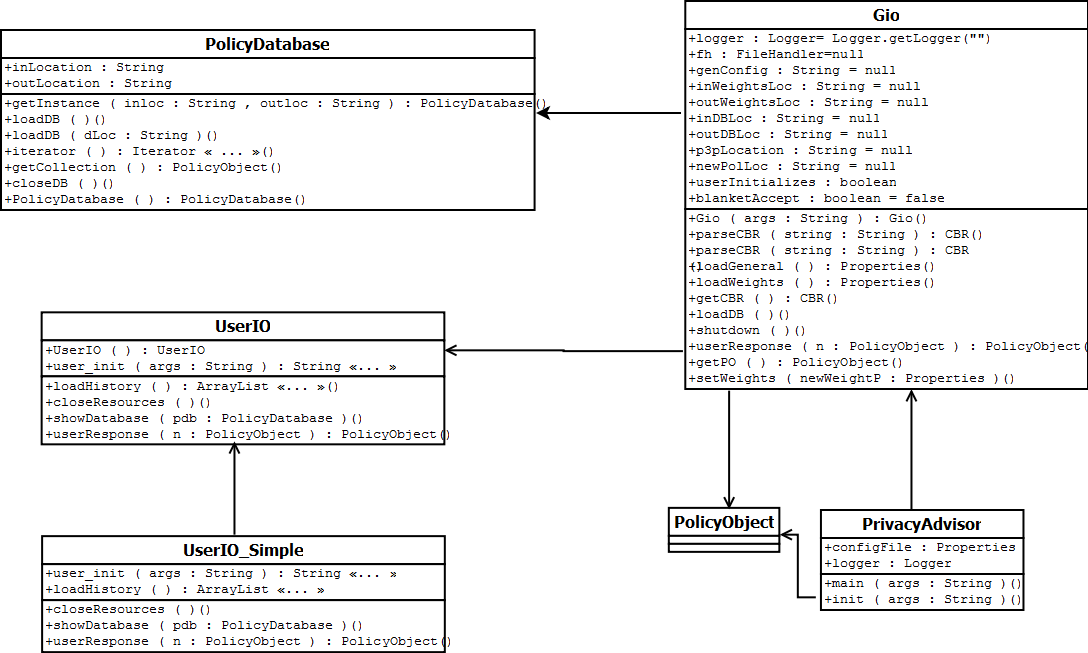
\includegraphics[width = \textwidth]{DesignReport/uml/gio.png}
\caption{Input/output and user interfaces.}
\label{UserIO}
\end{center}
\end{figure}


\begin{figure}[htbp]
\begin{center}
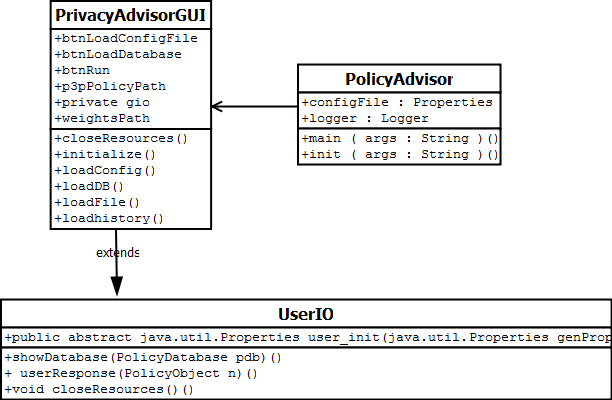
\includegraphics[width = \textwidth]{DesignReport/uml/policyadvisorgui}
\caption{GUI interfaces.}
\label{GUI_interface}
\end{center}
\end{figure}



\subsection{Community Server} %%TODO needs rewrite- focuse here is on design not implementation. mention query should be server-side
The community knowledge repository is implemented using a public CouchDB (no-SQL server), which is accessed using standard Java to JSON java libraries. The client program (end-user java application) communicates with the server at two points- when the application has insufficient knowledge, or confidence in its knowledge, to make a suggestion as to the acceptance of a new P3P policy; and after the user has confirmed or overridden the policy.

In the first instance, the new policy under consideration is converted to JSON using GSON (the Google Json libraries), and transmitted to the database, which parses the new policy and replies with a JSON encoded suggested Action.

In the second instance, the final policy (including the action taken on it) is sent to the CouchDB server, and the server proceeds to store the object.
On the database end, there are two essential interfaces (beyond any standard initialization and shutdown procedures). As seem above, these two interfaces are the suggestion provider, which includes a query to find the most similar policies and actions on them by the community, and a interface to simply save the new policy to the appropriate database.
The database is easily replaceable, requiring only the construction of a new class implementing 'NetworkR', the abstract class detailing the methods called by the PrivacyAdvisor framework. The selection between available 'NetworkR' implementations in made by setting the 'NetworkRType' configuration variable during initialization to the full classname.
